\documentclass[12]{article}
%\usepackage[utf8]{inputenc}
\usepackage{mathtools, amssymb, extarrows, bm}
\usepackage{tikz}
\usepackage{pgfplots}
\usepackage{setspace}
\usepackage[shortlabels]{enumitem}
\usepackage{hyperref}
\hypersetup{
	colorlinks=true,
	linkcolor=blue,
	filecolor=magenta,      
	urlcolor=cyan,
	pdftitle={Overleaf Example},
	pdfpagemode=FullScreen,
}
\usepackage{geometry}
\geometry{
	a4paper,
	total={140mm,257mm},
	left=35mm,
	top=20mm,
}
\usepackage{subcaption}
\usepackage{graphicx}
\usepackage{float}
\usepackage{import}

\newcommand{\myskip}{0.7em}
\newcommand{\prob}{{\mathbb P}}
\newcommand{\E}{{\mathbb E}}
\newcommand{\Var}{\mathrm{Var}}
\newcommand{\Cov}{\mathrm{Cov}}
\newcommand{\Corr}{\mathrm{Corr}}
%\renewcommand\thesection{Q\arabic{section}}
\pgfplotsset{
	standard/.style={%Axis format configuration
		axis x line=middle,
		axis y line=middle,
		enlarge x limits=0.15,
		enlarge y limits=0.15,
		every axis x label/.style={at={(current axis.right of origin)},anchor=north west},
		every axis y label/.style={at={(current axis.above origin)},anchor=north east},
		every axis plot post/.style={mark options={fill=white}}
	}
}

%%%%%%%%%%%%%%%%%%%%%%%%%%%%%%%%%%%%%%%%%%%%%%%%%%%%%%%%%%%%%%%%%%%%%%%%%%%%
\title{
	{\LARGE Security and Privacy in Machine Learning}\\
	{\Large Homework 1}\\
	{\normalsize Spring 2023}
}
\author{Javad Hezareh\\{\small 98101074}}
\date{}

\onehalfspacing
\begin{document}
	\maketitle
	\vspace{15mm}
	\tableofcontents
	
	\pagebreak
	\section{Cost Function}
	\begin{enumerate}[label=\textbf(\alph*)]
		\item
		Considering the MAE loss function and $f_\theta(x)$ we have:
		\[
		\begin{aligned}
			\mathcal{L}(\theta) &= \frac{1}{3} \left(|3-\theta^2+\theta| + |0-2\theta^2+2\theta| + |6 - 3\theta^2 + 3\theta|\right) \\[\myskip]
				&= \frac{|\theta^2-\theta-3| + 2|\theta^2-\theta| + 3|\theta^2-\theta-2|}{3}
		\end{aligned}
		\]
		For the graph of $\mathcal{L}(\theta)$ we have:
		\[
		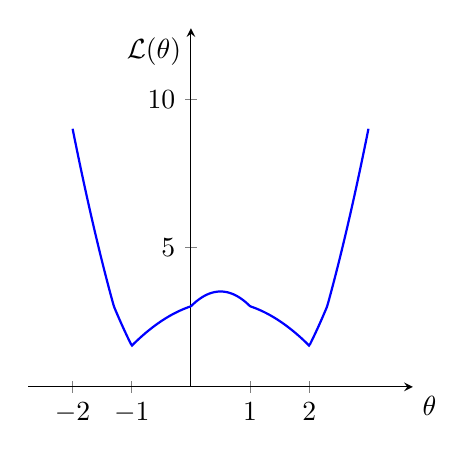
\begin{tikzpicture}
			\begin{axis}[
				scale=0.8,
				unit vector ratio*=2 1 1,
				standard,
				ymax=11,
				xtick={-2,-1,0,1,2},
				xlabel=\(\theta\),
				ylabel={\(\mathcal{L}(\theta)\)}
				]
				\addplot [thick,blue,domain=-2:3,samples=250] {abs(x*x-x-3)/3+2*abs(x*x-x)/3+abs(x*x-x-2)};
			\end{axis}
		\end{tikzpicture}
		\]
		Candidate points for minimum are $2$ and $-1$ where the value of the loss function is $\mathcal{L}(2)=5/3$ and $\mathcal{L}(-1)=5/3$. Therefore both of them are the local and global minima of $\mathcal{L}$. If we choose our learning rate enough small, then starting from any point on $\theta$ and using gradient descent algorithm we will end up on $2$ or $-1$ (depend on the starting point) which both of them are global minima, therefore using small enough learning rate will always lead us to the global minima of this loss function.
		\item
		Using MSE loss function and $f_\theta(x) = \ln(1+e^{x\theta})$ we have:
		\[
		\begin{aligned}
			\mathcal{L}(\theta) &= \frac{1}{3} \left[(0-\ln(1+e^\theta))^2 + (3-\ln(1+e^{-\theta}))^2 + (4-\ln(1+e^{3\theta}))^2\right]
		\end{aligned}
		\]
		Therefore the graph of $\mathcal{L}$ will be:
		\[
		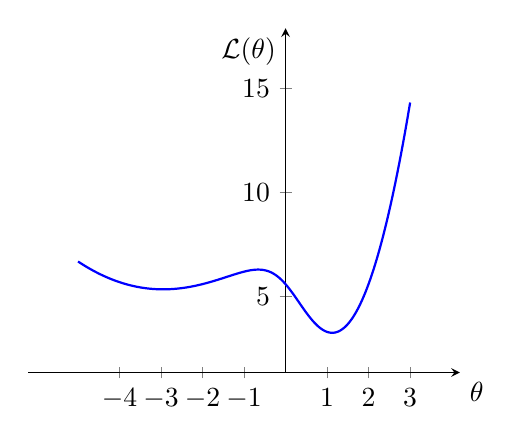
\begin{tikzpicture}
			\begin{axis}[
				scale=0.8,
				unit vector ratio*=2 1 1,
				standard,
				ymax=16,
				xtick={-4,-3,-2,-1,0,1,2,3},
				xlabel=\(\theta\),
				ylabel={\(\mathcal{L}(\theta)\)}
				]
				\addplot [thick,blue,domain=-5:3,samples=250] {(ln(1+exp(x))^2 + (3-ln(1+exp(-x)))^2 + (4-ln(1+exp(3*x)))^2)/3};
			\end{axis}
		\end{tikzpicture}
		\]
		So $\theta=-3$ will be a local minima with value $\mathcal{L}(-3)=?$, and $\theta=1$ will be the global minima with value $\mathcal{L}(1)=?$. In contrast to the previous part, using gradient descent in this setup will not always converge to the global minima and it depends on the starting point. For example if we start from a point less than $-3$ it will converge to $\theta=-3$ which is not the global minima.
		\item
		In deep networks we expect to have a lot of global and local minima where local minima points are not necessarily global as well. One solution to find the global minima is to use stochastic gradient descent which will allow us to skip some local minimas.
	\end{enumerate}

	\pagebreak
	\section{Training Model}
	\begin{enumerate}[label=\textbf{(\alph*)}]
		\item
		Performing normalization on input data will help the logistic regression model to avoid vanishing gradient and therefore converge faster. It will also help to increase the accuracy of the model a bit. Also, if we don't perform normalization, we can't interpret the coefficients as indicators of feature importance. Because we need to have the same scaling for different features to be able to compare coefficients norm.
		\item
		Using regularization in this model will help us to reach a better model in the sense of generalization error and performance.		
		\item
		A network with linear activation has no difference with a linear model. So using a 20 layer network with linear activation function will lead to a simple linear model which is not capable of capturing complex patterns in different data. On the other hand a 3 layer non-linear network has this ability to model the non-linearity and capture complex patterns as well. The later one will also has much less weights and parameters, and therefore is more computation efficient (in case of efficient calculation of non-linearity).
	\end{enumerate}
	
	\pagebreak
	\section{Perceptron Network}
	\begin{enumerate}[label=\textbf{(\alph*)}]
		\item
		This is not possible to classify the given points with just one line. At least we need to line to be able to do so.
		\item
		We will use two hyperplane crossing from the center of our data and then if one point be in the right side of both of them, then that point will be classified as class 1 and else as class 0.
		\begin{figure}[H]
			\centering
			\includegraphics[width=0.65\textwidth]{q3.png}
		\end{figure}
		For each point on line 1 such as $(x_1, x_2)$ we have $(-1,1)\cdot(x_1, x_2) + 2.5 = 0$, therefore for each point on the right side of this line we have $w_1\cdot x + 2.5 > 0$ where $w_1 = (-1, 1)$. For each point on line 2 such as $(x_1, x_2)$ we have $(1,1)\cdot(x_1, x_2) - 3.5 = 0$, therefore for each point on the right side of this line we have $w_2\cdot x - 3.5 > 0$ where $w_2 = (1,1)$. Hence we can use following networks to find out the relative position of each point respect to each line: (all activation functions are threshold)
		\vspace*{1.5em}
		\[
		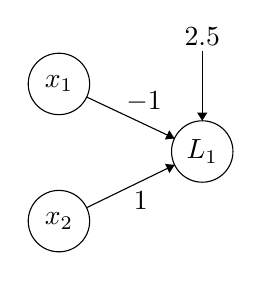
\begin{tikzpicture}[scale=0.13]
			\tikzstyle{every node}+=[inner sep=0pt]
			\draw [black] (22.6,-25.3) circle (3);
			\draw (22.6,-25.3) node {$x_1$};
			\draw [black] (22.6,-38.7) circle (3);
			\draw (22.6,-38.7) node {$x_2$};
			\draw [black] (36.6,-31.9) circle (3);
			\draw (36.6,-31.9) node {$L_1$};
			\draw [black] (25.31,-26.58) -- (33.89,-30.62);
			\fill [black] (33.89,-30.62) -- (33.38,-29.83) -- (32.95,-30.73);
			\draw (30.91,-28.09) node [above] {$-1$};
			\draw [black] (25.3,-37.39) -- (33.9,-33.21);
			\fill [black] (33.9,-33.21) -- (32.96,-33.11) -- (33.4,-34.01);
			\draw (30.59,-35.81) node [below] {$1$};
			\draw [black] (36.6,-22.1) -- (36.6,-28.9);
			\draw (36.6,-21.6) node [above] {$2.5$};
			\fill [black] (36.6,-28.9) -- (37.1,-28.1) -- (36.1,-28.1);
		\end{tikzpicture}
		\qquad \qquad
		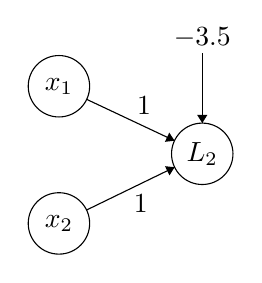
\begin{tikzpicture}[scale=0.13]
			\tikzstyle{every node}+=[inner sep=0pt]
			\draw [black] (22.6,-25.3) circle (3);
			\draw (22.6,-25.3) node {$x_1$};
			\draw [black] (22.6,-38.7) circle (3);
			\draw (22.6,-38.7) node {$x_2$};
			\draw [black] (36.6,-31.9) circle (3);
			\draw (36.6,-31.9) node {$L_2$};
			\draw [black] (25.31,-26.58) -- (33.89,-30.62);
			\fill [black] (33.89,-30.62) -- (33.38,-29.83) -- (32.95,-30.73);
			\draw (30.91,-28.09) node [above] {$1$};
			\draw [black] (25.3,-37.39) -- (33.9,-33.21);
			\fill [black] (33.9,-33.21) -- (32.96,-33.11) -- (33.4,-34.01);
			\draw (30.59,-35.81) node [below] {$1$};
			\draw [black] (36.6,-22.1) -- (36.6,-28.9);
			\draw (36.6,-21.6) node [above] {$-3.5$};
			\fill [black] (36.6,-28.9) -- (37.1,-28.1) -- (36.1,-28.1);
		\end{tikzpicture}
		\]
		Now with the following network we can classify data points:
		\[
		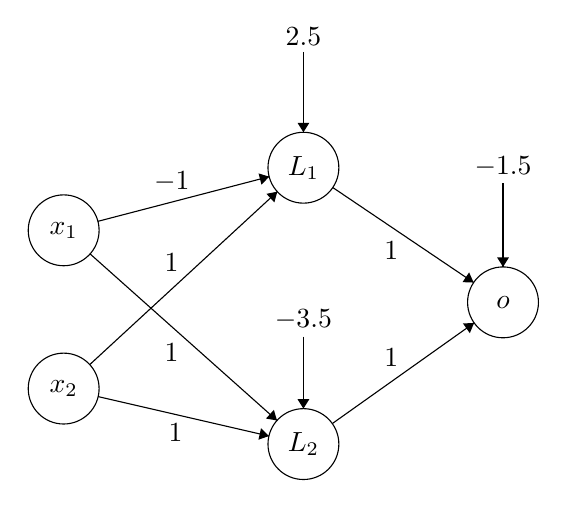
\begin{tikzpicture}[scale=0.15]
			\tikzstyle{every node}+=[inner sep=0pt]
			\draw [black] (22.6,-25.3) circle (3);
			\draw (22.6,-25.3) node {$x_1$};
			\draw [black] (22.6,-38.7) circle (3);
			\draw (22.6,-38.7) node {$x_2$};
			\draw [black] (42.9,-20) circle (3);
			\draw (42.9,-20) node {$L_1$};
			\draw [black] (42.9,-43.4) circle (3);
			\draw (42.9,-43.4) node {$L_2$};
			\draw [black] (59.8,-31.4) circle (3);
			\draw (59.8,-31.4) node {$o$};
			\draw [black] (25.5,-24.54) -- (40,-20.76);
			\fill [black] (40,-20.76) -- (39.1,-20.48) -- (39.35,-21.44);
			\draw (31.75,-22.06) node [above] {$-1$};
			\draw [black] (24.81,-36.67) -- (40.69,-22.03);
			\fill [black] (40.69,-22.03) -- (39.77,-22.21) -- (40.44,-22.94);
			\draw (31.73,-28.86) node [above] {$1$};
			\draw [black] (42.9,-10.2) -- (42.9,-17);
			\draw (42.9,-9.7) node [above] {$2.5$};
			\fill [black] (42.9,-17) -- (43.4,-16.2) -- (42.4,-16.2);
			\draw [black] (24.84,-27.3) -- (40.66,-41.4);
			\fill [black] (40.66,-41.4) -- (40.4,-40.5) -- (39.73,-41.24);
			\draw (31.74,-34.84) node [below] {$1$};
			\draw [black] (25.52,-39.38) -- (39.98,-42.72);
			\fill [black] (39.98,-42.72) -- (39.31,-42.06) -- (39.09,-43.03);
			\draw (32.08,-41.63) node [below] {$1$};
			\draw [black] (42.9,-34.3) -- (42.9,-40.4);
			\draw (42.9,-33.8) node [above] {$-3.5$};
			\fill [black] (42.9,-40.4) -- (43.4,-39.6) -- (42.4,-39.6);
			\draw [black] (45.39,-21.68) -- (57.31,-29.72);
			\fill [black] (57.31,-29.72) -- (56.93,-28.86) -- (56.37,-29.69);
			\draw (50.35,-26.2) node [below] {$1$};
			\draw [black] (45.35,-41.66) -- (57.35,-33.14);
			\fill [black] (57.35,-33.14) -- (56.41,-33.19) -- (56.99,-34.01);
			\draw (50.35,-36.9) node [above] {$1$};
			\draw [black] (59.8,-21.3) -- (59.8,-28.4);
			\draw (59.8,-20.8) node [above] {$-1.5$};
			\fill [black] (59.8,-28.4) -- (60.3,-27.6) -- (59.3,-27.6);
		\end{tikzpicture}
		\]
	\end{enumerate}
	
	\pagebreak
	\section{Softmax and Cross-Entropy}
	By substituting the softmax function in our loss we have:
	\[
	\mathcal{L}(\bm{\hat{y}}, \bm{y}) = - \sum_{i=1}^{M} y_i \log \left(\frac{e^{x_i}}{\sum_{m=1}^{M}e^{x_m}}\right) = - \sum_{i=1}^{M} y_i\left(x_i - \log\left(\sum_{m=1}^{M}e^{x_m}\right)\right)
	\]
	Now for the derivative of loss w.r.t $x$ we have:
	\[
	\begin{aligned}
		\frac{\partial \mathcal{L}(\bm{\hat{y}}, \bm{y})}{x_j} &= -\sum_{i=1}^{M} y_i \frac{\partial}{\partial x_j} \left(x_i - \log\left(\sum_{m=1}^{M}e^{x_m}\right)\right) \\[\myskip]
		&= -\sum_{i=1}^{M} y_i \left(1_{i=j} - \frac{e^{x_j}}{\sum_{m=1}^{M}e^{x_m}}\right)
	\end{aligned}
	\]
	If we assume that $y_i$s are probability distribution, then they will sum up to $1$ and hence we have:
	\[
	\begin{aligned}
		& \frac{\partial \mathcal{L}(\bm{\hat{y}}, \bm{y})}{x_j} = - y_j + \frac{e^{x_j}}{\sum_{m=1}^{M}e^{x_m}} = -y_j + \hat{y}_j \\[\myskip]
		\implies & \boxed{\frac{\partial \mathcal{L}(\hat{y}, y)}{\bm{x}} = \bm{\hat{y}} - \bm{y}}
	\end{aligned}
	\]
	
	\pagebreak
	\section{Backpropagation}
	\begin{enumerate}[label=\textbf{(\alph*)}]
		\item
		If we assume the middle layer has $p$ neuron, then we have:
		\[
		\begin{dcases}
			\bm{W_1} \in \mathbb{R}^{p\times n} \\
			\bm{b_1} \in \mathbb{R}^{p\times 1} \\
			\bm{W_2} \in \mathbb{R}^{1\times p} \\
			\bm{b_2} \in \mathbb{R}
		\end{dcases}
		\]
		\item
		Let's assume that $\bm{X} \in \mathbb{R}^{n\times b}$ where $b=2000$. Then this will not change the weigh matrices and we only need to copy biases in $b$ columns. Therefore:
		\[
		\begin{dcases}
			\bm{W_1} \in \mathbb{R}^{p\times n} \\
			\bm{b_1} \in \mathbb{R}^{p\times b} \\
			\bm{W_2} \in \mathbb{R}^{1\times m} \\
			\bm{b_2} \in \mathbb{R}^{1\times b}
		\end{dcases}
		\]
		\item
		Let's derive this formulas for one data point, in other words $\bm{x}$ is not a batch of inputs.
		
		For $\partial \bm{z_1}/\partial \bm{W_1}$, we need to find the partial derivative of each element of $\bm{z_1}$ with respect to each element of $\bm{W_1}$. But we know ${z_1}_k$ only depends on the $k$-th row of $\bm{W_1}$, so $\partial {z_1}_k / \partial {W_1}_{ij} = 0$ if we have $k \ne i$. In case of $k = i$ then ${z_1}_k$ is the inner product of $k$-th row of $\bm{W_1}$ and $\bm{x}$, therefore $\partial {z_1}_k / \partial {W_1}_{ij} = x_j$ if $k = i$. So we have:
		\[
		\frac{{z_1}_k}{{W_1}_{ij}} = \begin{dcases}
			0 & k \ne i \\
			x_j & k = i
		\end{dcases}
		\]
		For $\partial{\bm{a_1}}/\partial{\bm{z_1}}$, as ${a_1}_i$ only depends on ${z_1}_i$, we have:
		\[
		\frac{\partial{a_1}_i}{\partial{z_1}_j} = \begin{dcases}
			0 & i \ne j \\
			1 & i = j \;\;\text{and}\;\; {z_1}_j \ge 0 \\
			a & i = j \;\;\text{and}\;\; {z_1}_j < 0
		\end{dcases} 
		\]
		From the network architecture we know that $z_2$ is an scalar and hence we have:
		\[
		\frac{\partial z_2}{\partial \bm{a_1}} = \bm{W_2}^T
		\]
%		For $\partial\bm{z_2}/\partial\bm{a_1}$, as we know ${z_2}_i$ is the inner product of the $i$-th row of $\bm{W_2}$ and $\bm{a_1}$, then we have:
%		\[
%		\frac{\partial {z_2}_i}{\partial {a_1}_j} = {W_2}_{ij} %\implies \frac{\partial \bm{z_2}}{\partial \bm{a_1}} = \bm{W_2}
%		\]
		
		Using sigmoid function derivative, for $\partial \hat{y}^{(i)} / \partial z_2$ we have:
		\[
		\frac{\partial \hat{y}^{(i)}}{\partial z_2} = \hat{y}^{(i)}(1-\hat{y}^{(i)})
		\]
		For the derivative of loss w.r.t $\hat{y}$ we have:
		\[
		\frac{\partial \mathcal{L}}{\partial \hat{y}^{(i)}} = \frac{1}{m} \log \left(\frac{1-\hat{y}^{(i)}}{\hat{y}^{(i)}}\right)
		\]
		
	\end{enumerate}

	\pagebreak
	\section{Regularization}
	\begin{enumerate}[label=\textbf{(\alph*)}]
		\item
		Using this regularization will make our algorithm to decrease the $l_2$-norm of the weigh vector to reach less loss value. Therefore it is called "weight decay".
		\item
		By differentiating with respect to $\bm{w}$ and find its zeros we can find the optimal $\bm{w}^\ast$:
		\[
		\begin{aligned}
			\frac{\partial}{\partial\bm{w}} \mathcal{L} &= \frac{1}{N} \frac{\partial}{\partial\bm{w}} \|X\bm{w} - y\|^2 + \lambda \frac{\partial}{\partial\bm{w}} \|\bm{w}\|^2
		\end{aligned}
		\]
		We can differentiate the first term by expanding the norm with inner product:
		\[
		\begin{aligned}
			\|X\bm{w}-y\|^2 &= (X\bm{w}-y)^T(X\bm{w}-\bm{y}) \\[\myskip]
				&= \|X\bm{w}\|^2 + \|\bm{y}\|^2 -2\bm{y}^TX\bm{w}
		\end{aligned}
		\]
		\[
		\begin{aligned}
			\implies \frac{\partial}{\partial \bm{w}} \|X\bm{w} - \bm{y}\|^2 = 2(X^TX) \bm{w} - 2(X^T\bm{y}) \\[\myskip]
		\end{aligned}
		\]
		Therefore we have:
		\[
		\begin{aligned}
			& \frac{\partial \mathcal{L}}{\partial \bm{w}} = \frac{(2X^TX - 2\lambda N \bm{I})\bm{w} - 2X^T\bm{y}}{N} \\[1.25em]
			\implies & \frac{(2X^TX - 2\lambda N \bm{I})\bm{w^\ast} - 2X^T\bm{y}}{N} = 0 \\[\myskip]
			\implies &\boxed{\bm{w^\ast} = (X^TX-\lambda N \bm{I})^{-1}X^T\bm{y}}
		\end{aligned}
		\]
		\item
		As we can see in the above formula for the optimal weight vector, we need to find the inverse of $X^TX-\alpha\bm{I}$. This might not be possible for all values of $\alpha$, for example if $\alpha$ be one of the eigenvalues of $X^TX$, then there won't be any inverse matrix and we can't use this formula to find the optimal weight vector.
	\end{enumerate}
\end{document}
